\scanpage{596}

as $\varepsilon'_3(\tau')a'=\alpha'^{-1}u'$ (61), the formula a \uline{little convoluted}:
\margin{Sic! Here is the monster that gave me cold sweats
\unsure{for} \unsure{a morning} or two!}
\[
\tag{65}
\alpha''=(\varepsilon u'(\alpha)\alpha')\mathbin{.}
\left[
\underbrace{\alpha'^{-1}u'}_{\substack{
\text{''}\\
\varepsilon'_3(\tau')a'\\
\rotatebox[origin=c]{-90}{$\in$}\\
\deleted{\unsure{Z_\rho|N_\rho}}
}},\ \varepsilon_3(\tau')
\right].
\]
(where $\varepsilon\in\{\pm1\}$ \unsure{defined in|definition} (63))

\unsure{It|I} remains to examine the question whether the extension
\deleted{of} $S_0^{\unsure{\Pi}}\Gamma_{\rho,\sigma}$ of
$Z^!_{\rho,\sigma}\simeq M^![0]$ by $\mu=\{\pm1\}$ is trivial or not,
taking into account the fact that its restrictions to $Z^{!'}_{\rho,\sigma}$ and to
$Z^{!'''}_{\rho,\sigma}$ are trivial.

Let $S_0^\Pi\Gamma^{!'}_{\rho,\sigma},\ S_0^\Pi\unsure{\Gamma|W}^{!'''}_{\rho,\sigma}$\unsure{)|]}
be the inverse images of $\unsure{Z}^{!'}_{\rho,\sigma},\ Z^{!'''}_{\rho,\sigma}$
in $S_0^\Pi\Gamma^!_{\rho,\sigma}$, hence
\[
\tag{66}
\left\{
\begin{aligned}
\unsure{S_0^\Pi|\Sigma_{\rho k}^{\Pi}}\Gamma^{!'}_{\rho,\sigma}
&=S_0^\Pi\Gamma^!_{\rho,\sigma}\cap\Gamma^{!'}_{\rho,\sigma}\\
S_0^\Pi\Gamma^{!'''}_{\rho,\sigma}
&=S_0^\Pi\Gamma^!_{\rho,\sigma}\cap\Gamma^{!'''}_{\rho,\sigma}
\end{aligned}
\right.
\]
and we have exact sequences of central extensions
\diagram{
\[
\tag{67}
\left\{\vcenter{\hbox{%
\begin{tikzcd}[ampersand replacement=\&,column sep=large,row sep=large]
1\arrow[r,dash]\&\mu\arrow[r]\&S_0^\Pi\Gamma^{!'}_{\rho,\sigma}\arrow[r]\&Z^{!'}_{\rho,\sigma}\arrow[r]\&1\\
1\arrow[r,dash]\&\mu\arrow[r]\&S_0^\Pi\Gamma^{!'''}_{\rho,\sigma}\arrow[r]\&Z^{!'''}_{\rho,\sigma}\arrow[r]\&1
\end{tikzcd}%
}}\right.,
\]
}
which are split by subgroups denoted respectively
$S_0^{\Pi_0}\Gamma^{!'}_{\rho,\sigma},\ S_0^{\Pi_0}\Gamma^{\unsure{!''|!'''}}_{\rho,\sigma}$,
so that we have
\[
\tag{68}
\left\{
\begin{aligned}
S_0^\Pi\Gamma^{!'}_{\rho,\sigma}
&\simeq S_0^{\Pi_0}\Gamma^{!'}_{\rho,\sigma}\times\mu\\
S_0^\Pi\Gamma^{!'''}_{\rho,\sigma}
&\simeq S_0^{\Pi_0}\Gamma^{!'''}_{\rho,\sigma}\times\mu.
\end{aligned}
\right.
\]
\mspage{595}

\scanpage{597}
\mspage{602}

I ask myself whether these subgroups
\[
(69)\qquad
\left\{
\begin{aligned}
S_0^{\Pi_0}\Gamma_{\rho,\sigma}^{!'}&\subset S_0^{\Pi}\Gamma_{\rho,\sigma}^{!'}\subset S_0^{\Pi}\Gamma_{\rho,\sigma}^{!}\\
S_0^{\Pi_0}\Gamma_{\rho,\sigma}^{!'''}&\subset S_0^{\Pi}\Gamma_{\rho,\sigma}^{!'''}\subset S_0^{\Pi}\Gamma_{\rho,\sigma}^{!}
\end{aligned}
\right.
\]
\margin{Subgroups \unsure{of indices|of index} $4$ in $S_0^{\Pi}\Gamma_{\rho,\sigma}$}
are \uline{invariant} in $S_0^{\Pi}\Gamma_{\rho,\sigma}^{!}$, which
would also mean (\unsure{passing} then to the quotient by these subgroups)
that the extension $S_0^{\Pi}\Gamma_{\rho,\sigma}^{!}$ of $Z_{\rho,\sigma}^{!}$
by $\mu$, split over $Z_{\rho,\sigma}^{!'}$ and over $Z_{\rho,\sigma}^{!'''}$,
in fact comes (with the said splittings) from extensions of
$Z_{\rho,\sigma}^{!}/Z_{\rho,\sigma}^{!'}\ (\simeq\pm1)$ and of
$Z_{\rho,\sigma}^{!}/Z_{\rho,\sigma}^{!'''}\ (\simeq\pm1)$ by $\mu$,
which would then have to be characterized (as trivial or nontrivial).

Since the subgroups in question are normal in
$S_0^{\Pi}\Gamma^{!'}$ resp. $S_0^{\Pi}\Gamma^{!'''}$, \deleted{and}
if $x$ is an element of $S_0^{\Pi}\Gamma^{!}$ which is
\uline{not} in $S_0^{\Pi}\Gamma^{!'}$ resp. $S_0^{\Pi}\Gamma^{!'''}$,
to say that $S_0^{\Pi_0}\Gamma^{!'}$ (resp. $S_0^{\Pi_0}\Gamma^{!'''}$)
is normal in $S_0^{\Pi}\Gamma^{!}$ \unsure{as a whole} simply means
that it is normalized by $x$.

$1^\circ)$ Case of $S_0^{\Pi_0}\Gamma^{!\unsure{'}}\deleted{\unsure{''}}$
in $S_0^{\Pi}\Gamma^{!}$. We shall take
\inserted{$\underline{x}=(u_0,a_0,b_0)$ with $u_0=\tau$, hence
$\varepsilon_3(u_0)=\varepsilon_2(u_0)=\unsure{\chi}(u_0)=-1$,}
\deleted{$x=\tau$, which is not in $S_0^{\Pi}\Gamma^{!'}$}
\[
(70)\qquad
\left\{
\begin{gathered}
\alpha_0=\tau,\quad \inserted{\beta_0=1,}\quad
\unsure{a_0}=\unsure{\varepsilon^0_{3,0}}(\tau')\alpha_0^{-1}u_0=\tau',
\quad b_0=\beta_0^{-1}u_0=\tau\big)\\
\text{thus}\qquad
\underline{x}=(\unsure{u_0}=\tau,\ a_0=\tau',\ b_0=\tau)
\end{gathered}
\right.
\]

\mspage{596}

\scanpage{598}

thus we have
\[
x\in S_0^{\Pi_0}\Gamma^{!'''}
\underset{2}{\subset}S_0^{\Pi}\Gamma^{\unsure{!}}
\deleted{\unsure{S_0^{\Pi}\Gamma^{!}}}
\quad\text{and}\quad x\notin S_0^{\Pi}\Gamma^{!'}
\]
and we must see whether $x$ normalizes $S_0^{\Pi_0}\Gamma^{!'}$.

Let \deleted{$\unsure{u\in}$}
\[
(71)\qquad
\underline{u}\deleted{\unsure{\in Z}}=
\left(
\underset{\inserted{\substack{\rotatebox{90}{$\in$}\\Z}}}{\unsure{u}},
\underset{\inserted{\substack{\rotatebox{90}{$\in$}\\N_\rho'}}}{a},
\underset{\inserted{\substack{\rotatebox{90}{$\in$}\\N_\sigma'}}}{b}
\right)\in S_0^{\Pi_0}\Gamma^{!'}
\quad\text{i.e.}\quad
\left\{\begin{aligned}
u&\equiv a\equiv b\quad(\Pi_0)\\
\varepsilon_3(u)&=1
\end{aligned}\right.
\]
and let us compute
\[
\underline{x}\,\underline{u}\,\underline{x}^{-1}
=\underline{x}\,\underline{u}\,x
=(\tau(u),\tau'(a),\tau(b))
\]
is it in $S_0^{\Pi_0}\Gamma'$ (it is \illegible{1} \unsure{only|certainly} in
$S_0^\Pi\Gamma'$) i.e. do we have
\[
\deleted{\unsure{(70)}}\quad(72)\qquad
\tau(u)\equiv\tau'(\unsure{a})\equiv
\tau^{\deleted{\unsure{'}}}(b)\quad(\Pi_0)\qquad ?
\]
The relation $\tau(u)\equiv\tau(b)\equiv\tau(a)$ is an immediate consequence of
(71), so (72) is equivalent to
\[
\tau'(a)\equiv\tau(a)\quad\inserted{(\Pi_0)}
\qquad(\text{i.e. }\sigma^{-1}(\tau(a))=\tau(a)
\]
i.e.
\[
(73)\qquad\unsure{\text{---}}\qquad
[\dot\sigma,\tau(a)^{\cdot}]=1
\quad\text{in }\unsure{\widetilde{\mathcal G}^{*}}/\Pi_0
\]
\margin{\uline{N.B.}}
Or again, \deleted{\unsure{obviously|equivalent}}, by virtue of (35 bis)
\deleted{\[
a=\underbrace{\varepsilon_3(\tau')}_{\substack{\uparrow\\1}}\alpha^{-1}u,
\quad\text{hence}\quad\tau(a)=\tau(\alpha)^{-1}\tau(u)
\]}
\[
\varepsilon_2(\tau(a))=1\qquad\text{i.e.}\quad\varepsilon_2(a)=1
\]
or finally (since $a\equiv u\ (\Pi_0)$)
\[
(74)\qquad\varepsilon_2(u)=\unsure{1}\,.
\]
This condition is not a consequence of the condition $\varepsilon_3(u)=1$,
which shows that $S_0^{\Pi_0}\Gamma^{!'}$ is not invariant in
$S_0^{\Pi}\Gamma^!$.

Is $S_0^{\Pi_0}\Gamma^{!'''}$ invariant in $S_0^{\Pi}\Gamma^!$?

Let \deleted{$x\in S_0$}
\[
(75)\qquad
x=(u_0,\unsure{a_0},b_0)\in S_0^{\Pi_0}\Gamma^{!'}
\mathbin{\setminus}S_0^{\Pi}\Gamma^{!'''}
\quad\text{thus}\quad
\begin{gathered}
\unsure{\text{a)}}\quad
\left\{\begin{aligned}
\varepsilon_3(u_0)&=1\\
\varepsilon_2(u_0)&=-1
\end{aligned}\right.\\
\deleted{\varepsilon_2(u_0)\varepsilon_3(u_0)=\unsure{-1|1}}\\
\text{b)}\quad u_0\equiv b_0\equiv a_0\quad(\Pi_0)
\end{gathered}
\]

\mspage{597}

\scanpage{599}
\mspage{603}

and let us study its action on
\[
(76)\qquad
\underline{u}=(u,a,b)\in S_0^{\Pi_0}\Gamma^{!'''}
\quad
\left\{\begin{aligned}
\text{a)}\quad
\underbrace{\unsure{\varepsilon_2}(u)}_{\inserted{\varepsilon_2}}
\underbrace{\varepsilon_3(u)}_{\inserted{\varepsilon_3}}&=1\\
\text{b)}\quad u\equiv\unsure{b}&\equiv
\unsure{\varepsilon_3}(\unsure{\sigma})a\quad(\widehat\Pi_0)
\end{aligned}\right.
\]

We have
\[
(77)\qquad
\underline{x}\,\underline{u}\,\underline{x}^{-1}
=(u_0(u),a_0(a),b_0(b))
\]
and the relation $\underline{x}\,\underline{u}\,\underline{x}^{-1}
\in S_0^{\Pi_0}\Gamma^{!'''}$ is written
\[
(78)\qquad
u_0(u)\equiv b_0(b)\equiv\varepsilon_3'(\sigma)\mathbin{.}a_0(a)\,.
\]
\margin{N.B. $\varepsilon_3(u_0(u))=\varepsilon_3(u)$}
Now the relations (75) b) and 76 b) immediately imply
\[
u_0(u)\equiv b_0(b)\equiv
\underbrace{a_0(\varepsilon_3(\sigma)\mathbin{.}a)}_{
\varepsilon_3[a_0(\sigma)]\mathbin{.}a_0(a)}
\]
thus the relation (78) is also equivalent to
\[
(79)\qquad
\varepsilon_3[\sigma]\equiv\varepsilon_3[a_0(\sigma)]
\]
which is automatically satisfied if $\varepsilon_3=1$, and for
$\varepsilon_3=-1$ amounts to
\[
(80)\qquad\sigma\equiv a_0(\sigma)\quad\unsure{(\widehat\Pi_0)}
\]
\[
\text{i.e.}\quad\varepsilon_2(a_0)=1\qquad
\text{i.e.}\quad\varepsilon_2(u_0)=1,
\]
a relation which is \uline{false} by hypothesis 75 a).

Thus we again find $S_0^{\Pi_0}\Gamma^{!'''}$ \unsure{non-invariant}
in $S_0^{\Pi}\Gamma^!$. On the other hand,
\deleted{\unsure{let us denote|let us define}}\inserted{let us set}
\deleted{by $\Gamma^0$ the}
\[
(81)\qquad
\left\{\begin{aligned}
S_0\Gamma^0
&=\operatorname{Ker}\bigl(S_0\Gamma^0
\xrightarrow{(\varepsilon_2,\varepsilon_3)}\mu\times\mu\bigr)
=S_0\Gamma^{!'}\cap S_0\Gamma^{\unsure{!'''}}\\
&\hspace{22em}=S_0\Gamma^{!'}\cap S_0\Gamma^{!''}\\
&\hspace{22em}=S_0\Gamma^{!''}\cap S_0\Gamma^{!'''}\\
S_0^{\Pi}\Gamma^0&=S_0\Gamma^{!0}\cap S_0^{\Pi}\Gamma^!,\\
S_0^{\Pi_0}\Gamma^0&=S_0\Gamma^{!0}\cap S_0^{\Pi_0}\Gamma^!,
\end{aligned}\right.
\]
\margin{\deleted{\unsure{b)}}}
so that we have an exact sequence
\[
(82)\qquad
\diagram{\begin{tikzcd}[ampersand replacement=\&,column sep=large]
1\arrow[r,dash]\&\mu\arrow[r,dash]\&
S_0^{\unsure{\Pi|\Pi_0}}\Gamma^{\unsure{!0}}
\arrow[r]\&S_0\Gamma^{!0}\arrow[r]\&1
\end{tikzcd}},
\]

\mspage{598}

\scanpage{600}

canonically split by $S_0^{\Pi_0}\Gamma_0$ --- we therefore find
\[
(82)\qquad
S_0^{\Pi}\Gamma^{!0}=S_0^{\Pi_0}\Gamma^{!0}\times\mu\,.
\]

This being so, the preceding calculations show that
$S_0^{\Pi_0}\Gamma^{!0}$, which is of index $8$ in
$S_0^{\Pi}\Gamma^!$, is an invariant subgroup. In summary:

\uline{Proposition} Consider the subgroups
\inserted{(of indices $4,4,8$)}
\deleted{of}
$S_0^{\Pi_0}\Gamma^{!'},\ S_0^{\Pi_0}\Gamma^{!'''},\
S_0^{\Pi_0}\Gamma^{!0}$ of $S_0^{\Pi}\Gamma^!$ which are the images
\unsure{of the|of their} \inserted{homomorphic} restrictions
$Z^{!'},Z^{!'''},Z^{!0}$ of the set-theoretic section:
$A$ defined by (51) (52) of $S_0^{\Pi}\Gamma^!$ over
$Z=M[0]$ --- which is multiplicative on these subgroups,
and therefore defines splittings of the inverse images
$S_0^{\Pi}\Gamma^{\unsure{'|!'}},
S_0^{\Pi}\Gamma^{\unsure{'''|!'''}},
S_0^{\Pi}\Gamma^{\unsure{0|!0}}$
of \deleted{$\unsure{S_0^{\Pi}}$}
$Z^{!'},Z^{!'''},Z^{!0}$ in $S_0^{\Pi}\Gamma^!$:
\[
(83)\qquad
\begin{gathered}
S_0^{\Pi}\Gamma^{!'}\simeq
\deleted{\unsure{\mu}}S_0^{\Pi_0}\Gamma^{!'}\times\mu,\qquad
S_0^{\Pi}\Gamma^{!'''}=S_0^{\Pi_0}\Gamma^{!'''}\times\mu,\qquad
S_0^{\Pi}\Gamma^{!0}=S_0^{\Pi_0}\Gamma^{!0}\times\mu.
\end{gathered}
\]

\margin{\figure{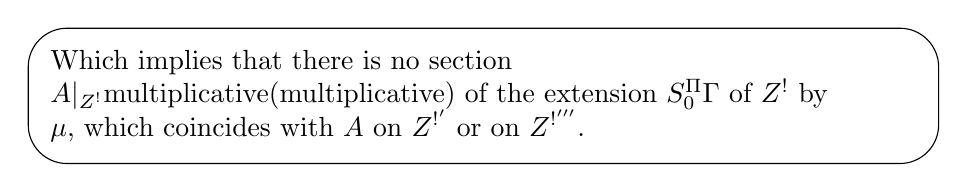
\begin{tikzpicture}
\node[draw,rounded corners=14pt,inner sep=8pt,text width=11cm,align=left]
{Which \unsure{implies} that there is no section
\deleted{$\unsure{A|_{Z^!}}$\unsure{multiplicative}}\inserted{(multiplicative)}
of the extension $S_0^{\Pi}\Gamma$ of $Z^!$ by $\mu$, which coincides
with $A$ on $Z^{!'}$ or on $Z^{!'''}$.};
\end{tikzpicture}}}

We then have this:

a) $S_0^{\Pi_0}\Gamma^{!'},S_0^{\Pi_0}\Gamma^{!'''}$ are
\uline{not} \uline{normal} in $S_0^{\Pi}\Gamma^!$.

b) $S_0^{\Pi_0}\Gamma^{!0}$ is normal in
$S_0^{\Pi}\Gamma^!$, so that the extension
$S_0^{\Pi}\Gamma^!$ of $Z^!\simeq M^![0]$ by $\mu$
is canonically isomorphic to the inverse image of an
\unsure{extension|category} \inserted{central} and finite
$S_0^{\Pi}\Gamma^!/(S_0^{\Pi_0}\Gamma^{!0})$
of $Z^!/Z^{!0}\simeq\mu\times\mu$ by $\mu$.

\mspage{599}